\documentclass{article}
\usepackage{graphicx}
\usepackage[margin=2cm]{geometry}
\usepackage[hidelinks]{hyperref}
\usepackage{color}

\begin{document}

\begin{titlepage}
  \begin{center}
    \huge
    \itshape\bfseries%Aplica estilo italico y negrita a todo el contenido agrupado
    Proyecto Moogle!\\
    \medskip
    Víctor Manuel Vena Barrios , C-113\\
    \medskip
    7 de mayo de 2023\\
    \vspace{5cm}
    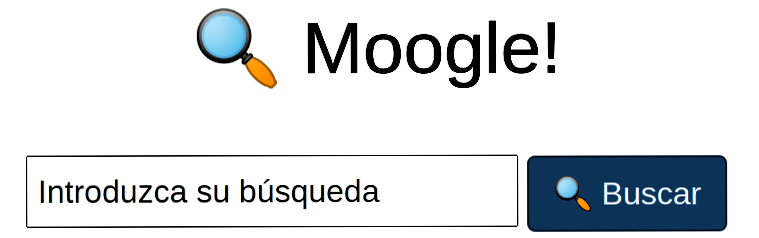
\includegraphics[scale=0.5]{Imagenes/moogle.png}
  \end{center}
\end{titlepage}

%crea automaticamente el indice
\tableofcontents

\section{Para ejecutar mi programa}
  \begin{enumerate}
    \item Crear en la carpeta del proyecto una carpeta llamada "Content" en la que debe poner los documentos
      \begin{itemize}
        \renewcommand{\labelitemi}{$\diamond$}
        \item Cada documento debe ser de extensión ".txt" y su nombre debe ser algo como\\
        palabras\_en\_minusculas\_separadas\_por\_guiones\_bajos.txt
      \end{itemize} 
    \item Abrir un terminal en la carpeta del proyecto
    \item Ejecutar el comando "make dev"
      \begin{itemize}
        \renewcommand{\labelitemi}{$\diamond$}
        \item De no tener la herramienta make ejecutar el comando "dotnet run --project MoogleServer"
      \end{itemize}
    \item Mientras presiona "Ctrl" de clic donde dice "http://localhost:5285", esto abrirá una página web en su navegador donde puede buscar
  \end{enumerate}
\begin{center}
  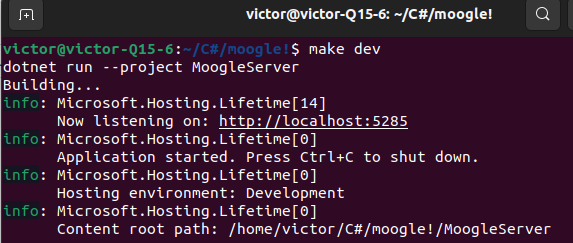
\includegraphics[scale=0.80]{Imagenes/Ejecutar_moogle.png}
\end{center}

\section{Funcionalidades}
\begin{itemize}
  \renewcommand{\labelitemi}{$\diamond$}
  \item Realiza buenas búsquedas. No todas sus palabras son igual de relevantes, este moogle! reconoce las que sí los son. Para buscar escriba en el cuadro de diálogo su consulta y de clic en el botón buscar.
  \item Se muestran primero los resultados más relevantes para su búsqueda, así le es posible encontrar antes lo que le interesa, ahorrándose tiempo.
  \item Para los más curiosos, decidimos mantener la lista de resultados completa, así puede analizar su búsqueda en un contexto amplio y variado.
  \item Con cada resultado se muestra un pedazo del texto para que conozca acerca del contenido del mismo y pueda decidir que resultado elegir.
  \item Ignora archivos vacíos,o que no contengan números ni letras, porque no aportan nada a las consultas del usuario. Pruebe a poner un archivo como este en la carpeta Content, vera que no saldrá en ninguna consulta que haga pues ni siquiera pasa la fase de carga.\\
  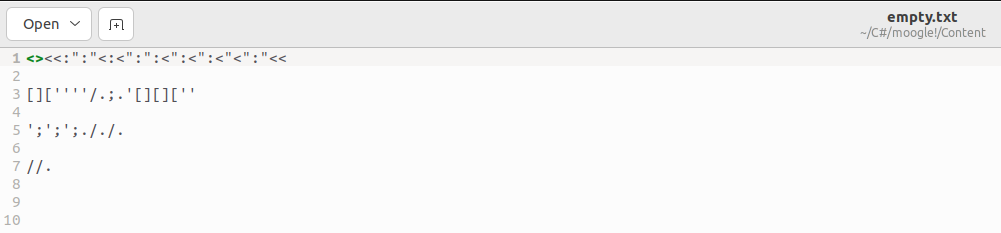
\includegraphics[scale=0.5]{Imagenes/Demostracion_de_Empty_._txt.png}
  \item Consideramos que usted es una persona y tiene derecho a equivocarse. Por eso ante cualquier eventualidad tipográfica le sugerimos una alternativa. Traducimos la consulta sin sentido "la casq" como "la casa". El muy común "algortmo" como "algoritmo". Usted debe copiar la sugerencia en el buscador y volver a buscar.
        \begin{center}
          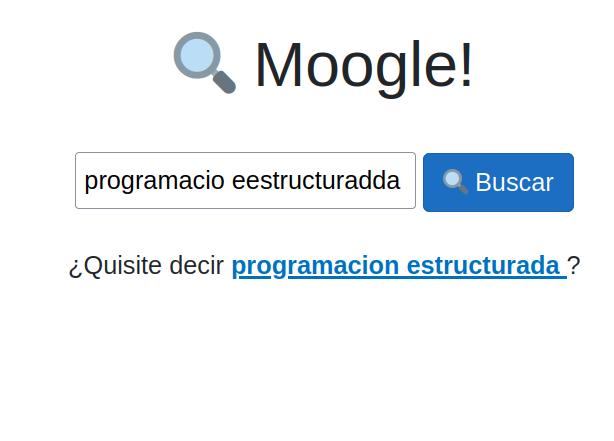
\includegraphics[scale=0.25]{Imagenes/programacion_estructurada.png}\\
        \end{center}
        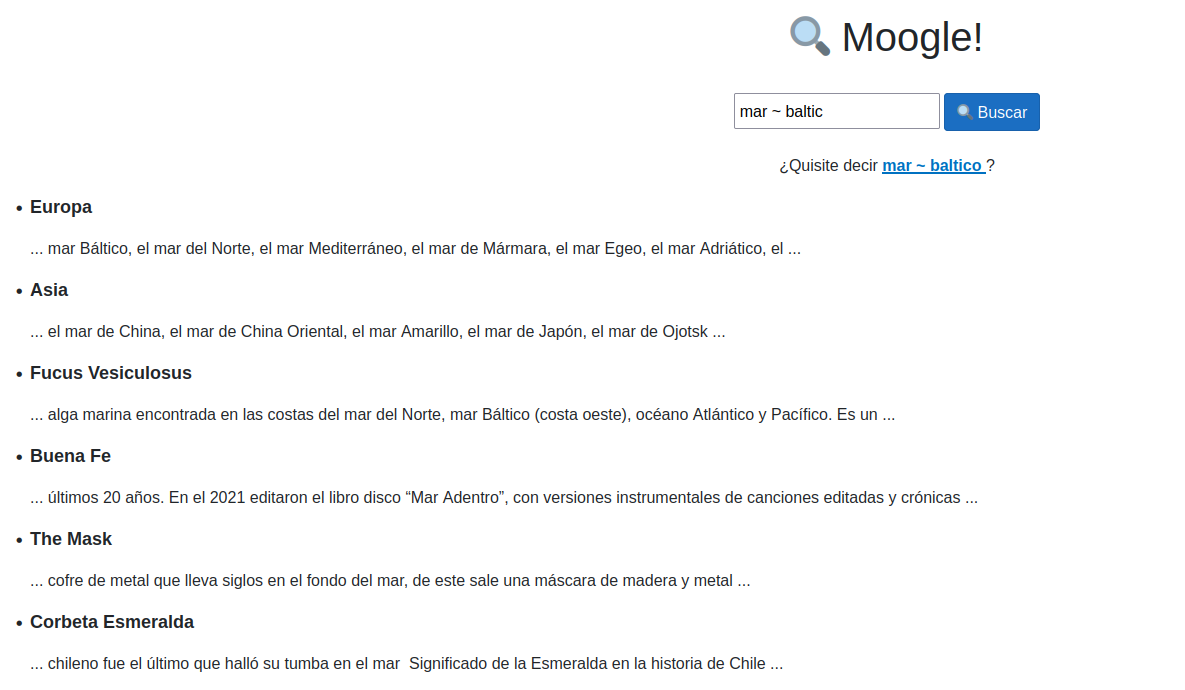
\includegraphics[scale=0.3]{Imagenes/mar_baltico_sugerencia.png}\\      
  \item Ahora es posible influenciar su búsqueda a través de varios símbolos, que llamamos operadores. Pruebe a buscar "Fama y fortuna".\\
    \begin{itemize}
      \item Utilice  \^{}  delante de las palabras que quiere que aparezcan en todos los resultados: "Fama y \^{}fortuna". 
      \item Utilice ! delante de las palabras que quiere que no aparezcan en ningún resultado "Fama y !fortuna".\\
      \includegraphics[scale=0.3]{Imagenes/newton\_con\_fama\_y\_sin\_fortuna.png}
      \item Utilice * delante de las palabras  que considere más importantes, se priorizarán los resultados que contengan estas palabras. Mientras más * más importancia . "Fama y ***fortuna".
      \item Utilice \~{} entre dos palabras que quiere que aparezcan cerca. Se priorizarán los resultados donde aparezcan cerca. "algoritmo \~{} bernoulli".\\
        \includegraphics[scale=0.3]{Imagenes/algoritmo\_bernoulli\_sin\_cercania.png}\\
        \includegraphics[scale=0.3]{Imagenes/algortimo\_bernoulli\_con\_cercania.png}
      \item También hemos hecho posible la combinación de operadores, a través de la precedencia. Por ejemplo, pruebe a consultar "alfa  beta", luego "\^{}alfa \^{}beta", y por ultimo "\^{}alfa \~{} \^{}beta".\\
      La regla es simple de recordar : 
      \begin{enumerate}
        \item Primero se aplican los operadores ! \^{} *, y solo el más cercano a la palabra. Por ejemplo la consulta "!!\^{}**\^{}perro \~{} !!*****gato",  es interpretada como "\^{}perro \~{} *****gato". Recordar que una secuencia de * se mantiene juntos.
        \item Luego se aplica el operador cercanía.
      \end{enumerate}
      Esto posibilita consultas del tipo "\^{}alfa \~{} \^{}beta": Muestra solo resultados donde estén alfa y beta, y prioriza en los que estén cerca.\\
      {\bfseries No existe un comportamiento definido para consultas contradictorias}: "\^{}ser o no !ser". Aplicar estos operadores mutuamente exclusivos a un mismo término no tiene un comportamiento definido, sea razonable.
    \end{itemize}
\end{itemize}

{\bfseries El contenido de la siguiente sección no es necesario para usar el programa.}

\section{Detalles Técnicos}

Utilicé un total de 144 documentos con un peso en conjunto de 12.6 Mb. Están almacenados en la carpeta Content en el directorio del programa y es posible añadir nuevos archivos para que se muestren en consulta. De eliminar todos los archivos de la carpeta Content o solamente dejar archivos vacíos , o sin palabras ni números, al iniciarse una búsqueda se lanzará una excepción con una advertencia para los desarrolladores.
\\
Mi código esta agrupado bajo el namespace MoogleEngine y estructurado en diferentes clases:
\begin{enumerate}
  \item Cargador: se encarga de cargar los archivos desde el disco duro.
	\item Coleccion: representa la colección de documentos, el corpus.
	\item Depurador: se encarga de eliminar resultados de la búsqueda considerados irrelevantes.
	\item Documento: representa un documento individual.
	\item Moogle: es el punto de entrada del código e implementa la lógica de la aplicación.
	\item Regla: almacena información relacionada con los operadores utilizados en la consulta y 	provee métodos auxiliares para aplicar los operadores.
	\item SearchItem: representa información acerca de los distintos documentos que responden a la 	búsqueda.
	\item SearchResult: representa el resultado de la búsqueda.
	\item Snippet: se encarga de computar el snippet de un documento.
	\item Sorter: se encarga de ordenar los resultados de la búsqueda basado en su relevancia.
	\item Sugerencia: se encarga de computar una sugerencia a partir de la consulta del usuario.
	\item Tokenizer: se encarga de procesar textos provenientes del usuario o de archivos.
	\item Valorador: se encarga de calcular el score de los documentos. Se encarga de lo relativo al 	modelo vectorial. Se encarga de aplicar los operadores utilizados por el usuario en la 	consulta.
	\item Vector: representa un documento como un vector.
\end{enumerate}

Conceptos claves: 
\begin{itemize}
  \item Término : Es cualquier secuencia finita de dígitos y/o letras. (son palabras , números, o una combinación)
  \item Archivo vacío : Archivo que no aporta información relevante al usuario. Esta vacío o no contiene ningún termino (ninguna letra o numero).
  \item Token Válido : Un token válido es un termino o uno de los operadores.
  \item Operadores : Uno de los símbolos ! \^{} * \~{}.
  \item Precedencia de los operadores:
        \begin{enumerate}
          \item De precedencia 1 o unarios: ! \^{} *
          \item De precedencia 2 o binarios : \~{}
        \end{enumerate} 
\end{itemize}

Como es el proceso de ejecución de una consulta? Cada vez que se realiza una consulta se llama al método Moogle.Query(string query). En este método se inicializa la colección de documentos, una vez por ejecución del programa y es en la primera consulta. Luego se procesa la consulta y se determinan los operadores que intervienen en ella, luego se calcula para cada documento un valor de relevancia respecto a la consulta y se aplican los operadores. Se crea por cada documento un resultado que contiene el valor de relevancia de dicho documento, su titulo y un pedazo de texto para mostrar. Se ordenan los resultados por relevancia. Se quitan los resultados irrelevantes. Se devuelve el listado de resultados y una sugerencia para la próxima consulta basada en esta. Para consultas sucesivas se sigue el mismo algoritmo, excepto que no se inicializa la colección.

Visualmente:
\begin{enumerate}
  \item Inicializar la colección si no ha sido inicializada. ( Coleccion.Inicializar )
    \begin{enumerate}
      \item Cargar los documentos. ( Cargador.Load )
        \begin{enumerate}
          \item Obtener los archivos de la carpeta Content.
          \item Crear un documento por cada archivo. ( Documento )
          \item Eliminar documentos vacíos.
        \end{enumerate}
      \item Asociar cada termino con los documentos en que aparece.
      \item Inicializar la Sugerencia con los términos. ( Sugerencia.Inicializar )
      \item Establecer la colección como inicializada.
    \end{enumerate}
  \item Procesar la consulta. ( Tokenizer.ProcesarQuery )
    \begin{enumerate}
      \item Separar la consulta en tokens. ( Tokenizer.Tokenize )
        \begin{enumerate}
          \item Normalizar los términos. ( Tokenizer.Normalizar )
        \end{enumerate}
      \item Actualizar Sugerencia. ( Sugerencia.Actualizar )
      \item Crear regla a partir de operadores. ( Regla )
      \item Eliminar StopWords.
    \end{enumerate}
  \item Calcular score. ( Valorador.Valorar )
    \begin{enumerate}
      \item Crear un vector a partir de la query y un vector a partir de cada documento. ( Vector )
      \item Aplicar operador * ( Regla.CalcularShould , Vector.AplicarOperador )
      \item Ignorar documentos que no cumplan con los operadores ! \^{} (  Regla , Documento.Contiene )
      \item Aplicar operador \~{} a vectores restantes( Regla.CalcularClose , Vector.AplicarOperador, Documento.Cercania )
      \item Calcular similaridad entre vectores. ( Valorador.SimilaridadCoseno , Vector * Vector )
    \end{enumerate}
  \item Crear resultados. ( SearchItem )
    \begin{enumerate}
      \item Cada resultado tiene asociado:
        \begin{itemize}
          \item Titulo ( Coleccion )
          \item Snippet ( Snippet.GetSnippet )
          \item Score
        \end{itemize}
    \end{enumerate}
  \item Ordenar resultados. ( Sorter.Sort )
  \item Depurar resultados. ( Depurador.Depurar )
  \item Devolver resultados  y Sugerencia( SearchResult, Sugerencia.Sugerir )
\end{enumerate}

Los elementos entre paréntesis constituyen los nombres de clases y métodos utilizados para realizar esta tarea. La anterior no es una descripción exhaustiva del funcionamiento del programa, aunque si capta la esencia del funcionamiento del mismo. Para profundizar  consulte la sección descripción de las clases más abajo.

\subsection{Descripcion de las clases}
\subsubsection{De la clase Cargador:}

El miembro contentDir establece de que directorio se cargaran los documentos. El directorio por defecto es el directorio Content. (En un futuro tener un archivo con un listado de directorios secundarios de donde también se carguen archivos).\\
El método Load() lee los archivos del disco duro. Lanza una excepción si no hay archivos que leer. Por cada archivo obtiene de el su contenido textual a través de ObtenElContenido(string nombreArchivo) y su titulo a través de ObtenElTitulo(string nombreArchivo) y crea un Documento(objeto de la clase Documento) a partir de esta información. Además determina la cantidad de documentos vacíos. Lanza una excepción si todos los documentos son documentos vacíos. Devuelve en un array los documentos no vacíos.\\
El método ObtenElContenido(string archivo) es una simple llamada al método File.ReadAllText(archivo).\\
El método ObtenElTitulo(string nombreArchivo) asumiendo que todos los archivos en la carpeta del contenido tienen un formato como el siguiente “palabras\_separadas\_por\_underscore\_y\_extension.txt” determina el título de los documentos. La forma de hacerlo está explicada en comentarios en el código.\\

\subsubsection{De la clase Colección:}
El miembro \_inicializada es utilizado para determinar si se debe realizar el proceso de inicialización o no.\\
El miembro \_documentos almacena los documentos que conforman la colección.\\
La propiedad Count es la cantidad de documentos en la colección.\\
La propiedad Documentos permite el acceso a los documentos de la colección.\\
El miembro terminosYApariciones asocia a cada termino de la colección los documentos en los que aparece.\\
El método Inicializar() llama al método Cargador.Load() que carga los diferentes archivos y devuelve un listado de documentos que se almacena en una variable de la clase Coleccion pues será utilizado posteriormente. Luego se asocia a cada término los documentos en los que aparece pues con esta información la clase Coleccion provee de métodos útiles. Luego se le pasa a la clase Sugerencia una copia de todos los términos presentes en la colección para que pueda aplicar posteriormente su algoritmo. Se establece Colección como inicializada de manera que en próximas llamadas al método Inicializar() se omitan todos estos pasos.\\
El método At(int index) devuelve una copia de el documento en determinada posición o lanza una excepción si la posición es inválida.\\
El método EnCuantosDocumentosAparece(string termino) devuelve la cantidad de documentos diferentes en los que aparece un término. Esta cantidad coincide con la cantidad de documentos asociados a dicho término en \_terminosYApariciones.\\
El método EsStopWord(string termino) determina si el termino dado es stop word en esta colección. Para ello empleo un criterio estadístico , un termino es stop word si aparece en al menos el 75\% del total de documentos.\\

\subsubsection{De la clase Depurador:}
El método Depurar(SearchItem[] items) se encarga de devolver solo los resultados que considere relevante. Para esto contamos la cantidad de elementos irrelevantes de items. Luego creo un nuevo array para la cantidad total de elementos menos los irrelevantes. Después relleno ese array con los elementos relevantes. Esto se hace con la ayuda del método auxiliar EsIrrelevante(SearchItem item)\\
El metodo EsIrrelevante(SearchItem item) determina si un resultado es relevante o no para la búsqueda basado en algún criterio. El utilizado por mi es que un resultado es irrelevante si su score es 0 o si tiene el valor NaN, valor que puede tener el tipo double para expresar que no es un número. La decisión de usar NaN se debe a que en ciertas búsquedas, carentes de términos por ejemplo, este valor apareció a la hora de calcular el score de varios documentos.\\

\subsubsection{De la clase Documento:}
El miembro \_terminos es un array de todos los términos del documento.\\
El miembro \_posicionEnTexto es la posición inicial que ocupa el i-ésimo termino de \_terminos en el  contenido textual del documento.\\
El miembro \_contenido asocia a cada termino las posiciones en \_termino donde aparece. Hay que notar que por la forma en que se construye el listado de posiciones asociadas a cada término es estrictamente creciente, lo cual nos será de utilidad más adelante.\\
El miembro \_mostFrequentTermCount almacena la cantidad de veces que se repite el término que más se repite y no es stop word. Es utilizado para calcular posteriormente por la clase Valorador el la frecuencia normalizada.\\
La propiedad Titulo es el título del documento.\\
La propiedad Texto es el contenido textual del documento. La diferencia entre Texto y \_terminos es que en Texto aparece cualquier símbolo, mientras que en \_terminos solo aparecen términos. Todo el contenido de \_terminos esta en Texto pero no sucede al revés.\\
La propiedad MostFrequentCount ofrece acceso al miembro \_mostFrequentTermCount y la primera vez que es llamada lo calcula.\\
La propiedad Contenido devuelve una copia de \_contenido.\\
La propiedad TerminosSinRepeticiones devuelve una copia del conjunto de los términos que conforman el documento.\\
La propiedad PosicionEnTexto devuelve una copia de \_posicionEnTexto.\\
La propiedad IsEmpty devuelve verdadero si el documento esta vacío, falso de otra forma. Un documento esta vacío si no contiene ningún termino.\\
El constructor Documento(string texto,string nombre) crea un Documento a partir de un archivo. Establece el Titulo como nombre y el Texto como texto. Utiliza el método Tokenizer.ProcesarTexto(string texto) para obtener el listado de términos de texto con el que establece \_terminos y las posiciones en el texto en las que aparecen los términos con el que establece \_posicionEnTexto. Luego inicializa \_mostFrequentTermCount en 0 e inicializa \_contenido asignando a cada termino de \_terminos las posiciones en que aparece.\\
El constructor Documento(Documento other) crea un documento a partir de copiar otro.\\
El método TermCount(string termino) devuelve la cantidad de apariciones de un termino en el documento o 0 si no aparece.\\
Los métodos Contiene(string termino) y NoContiene(string termino) se auxilian del método TermCount(string termino) para determinar si un termino aparece o no en el documento.\\
El método Cercania(string TerminoA,string TerminoB) determina la menor distancia entre los términos de entrada en el documento o -1 si alguno no aparece. Hay dos observaciones claves que hacer para entender como resolver este problema de forma eficiente, ya que es básico para implementar el operador de cercanía. La primera observación es que si mantenemos una posición fija y movemos la otra vemos que se comporta como una función modular, no negativa. La segunda observación es que como los listados de posiciones donde aparece cada termino son estrictamente crecientes, consideremos la siguiente situación:\\
TerminoA esta en la posición X1. TerminoB esta en la posición Y1. Supongamos sin perder generalidad que Y1 es la posición mayor. Sea Z1 la posición siguiente a Y1 , sabemos que Z1 $>$ Y1 por monotonía de los listados de posiciones. Por tanto se cumple que $Z1 – X1 > Y1 – X1$. Por lo que concluimos que elegir la posición siguiente al mayor es la peor opción que se puede considerar porque siempre aumenta la distancia , y por tanto disminuye la cercanía. Si se toma la posición siguiente al menor X1, sea esta W1. Puede suceder que $W1 < Y1$ , pero como $X1 < W1$ , $X1 – Y1 < W1 – Y1$, $Y1 – X1 > Y1 – W1$,en tal caso se minimiza la distancia. En el caso en que $W1 > Y1$ puede aumentar o disminuir la distancia dependiendo de las diferencias.\\
Propongo el siguiente algoritmo para calcular la cercanía:
\begin{verbatim}
    A = posiciones en que aparece TerminoA en el documento
    B = posiciones en que aparece TerminoB en el documento
    posicionActualA = primer elemento de A
    posicionActualB = primer elemento de B
    cercania = $\infty$
    Mientras(Queden elementos en A y Queden elementos en B)
        distancia = |posicionActualA – PosicionActualB|
        cercania = Minimo entre cercania y distancia
        Si posicionActualA <= PoscionActualB entonces PosicionActualA = siguiente elemento de A
        Si no posicionActualB = siguiente elemento de B
    Devolver cercania
\end{verbatim}

\subsubsection{De la clase Moogle:}
Esta clase solo contiene el método Query que está explicado anteriormente.

\subsubsection{De la clase Regla:}
El miembro \_not contiene los términos a los cuales se les aplico el operador ! en la consulta.\\
El miembro \_must contiene los términos a los cuales se les aplico el operador \^{} en la consulta.\\
El miembro \_should contiene los términos a los cuales se les aplico el operador * en la consulta y la cantidad de *.\\
El miembro \_close contiene las parejas de términos a los cuales se les aplico el operador ~ en la consulta.\\
Tiene un constructor por defecto que inicializa los miembros de datos.\\
Tiene un constructor que dado un listado de tokens inicializa los diferentes miembros.  Para ello realiza dos pasadas al listado de tokens, en la primera determina que operadores de precedencia 1 aplicar y los aplica. Para la segunda pasada considera solamente los términos y los operadores de cercanía, luego los aplica. Aplicar un operador quiere decir , en el caso del operador cercanía por ejemplo, almacenar la pareja de términos que tienen el operador en medio.\\
Tiene un constructor para crear una Regla a partir de otra, con una bandera que indica si es para snippet o no. Una regla para snippet solo considera los operadores * y \~{}, ya que estos pueden influir en qué pedazo de texto es más relevante para el usuario. Por ejemplo ,  si se aplica un operador cercanía a dos términos y como primer resultado aparece un documento que los contiene a una distancia 3, es deseable que en el snippet aparezca el pedazo de texto que los contiene a distancia 3.\\
Posee 4 propiedades que permiten el acceso a sus miembros de datos.\\
Tiene la propiedad IsEmpty que es verdadera en caso de que todos su miembros de datos estén vacíos, es decir, de no tener ningún operador que aplicar.\\
Los métodos EsOperador(string token) y EsTermino(string token) son auxiliares para la funcionalidad de la clase.\\
El método ToString() es sobrecargado para facilitar la depuración.\\
El método ParaSnippet() devuelve una copia de esta regla para utilizar en el cómputo de snippet. Se auxilia del constructor definido anteriormente.\\
Los métodos CalcularShould(int cantidadDeAsteriscos) y CalcularClose(int cercania) mantienen la lógica de los operadores dentro de la clase Regla. En ellos se implementan funciones que devuelven una valor multiplicativo usada para modificar los valores tf-idf de las componentes de algún vector.\\
El método CalcularShould(int cantidadDeAsteriscos) devuelve 1 + cantidad de asteriscos. Es una función lineal en la cantidad de asteriscos.\\
El metod CalcularClose(int cercania) es una función inversamente proporcional en la distancia entre dos términos dada por su cercanía. La cercanía de dos terminos solo puede ser positiva, por esto en caso contrario se devuelve 1, que al multiplicarse mantendrá neutro el resultado. Propongo la fórmula $1 + B / (cercania – A)$. Donde A y B son constantes establecidas en el programa. Esta fórmula siempre devuelve un resultado mayor o igual que 1, haciendo que en documentos donde aparezcan ambos términos relacionados por el operador cercanía vean un ascenso en su score, aunque sea mínimo. El valor de A debe ser tal que cuando la cercanía tienda a 1, su valor mínimo esperado, el valor de la función sea alto, no puede ser igual a 1 porque entonces ocurriría una división por 0. El valor elegido por mi es A = 0.9 .Recordemos que en una función inversamente proporcional el valor de A corresponde a la asíntota vertical donde el límite de la función tiende a infinito. El valor de B influye en la caída de valor de la función a medida que la cercanía aumenta. Elegí un valor de B = 1500, determinado de forma experimental para que la consulta “algoritmo ~ bernoulli” aparezca en primera posición con respecto a las demás que aparecen.\\
En la determinación de qué funciones utilizar me ha servido el conocimiento adquirido en el curso de Análisis Matemático, del cual estoy agradecido.\\
Ejemplo del comportamiento de la función de cercanía para distintos valores de B con A  = 0.9\\
\begin{center}
  B=1\\
  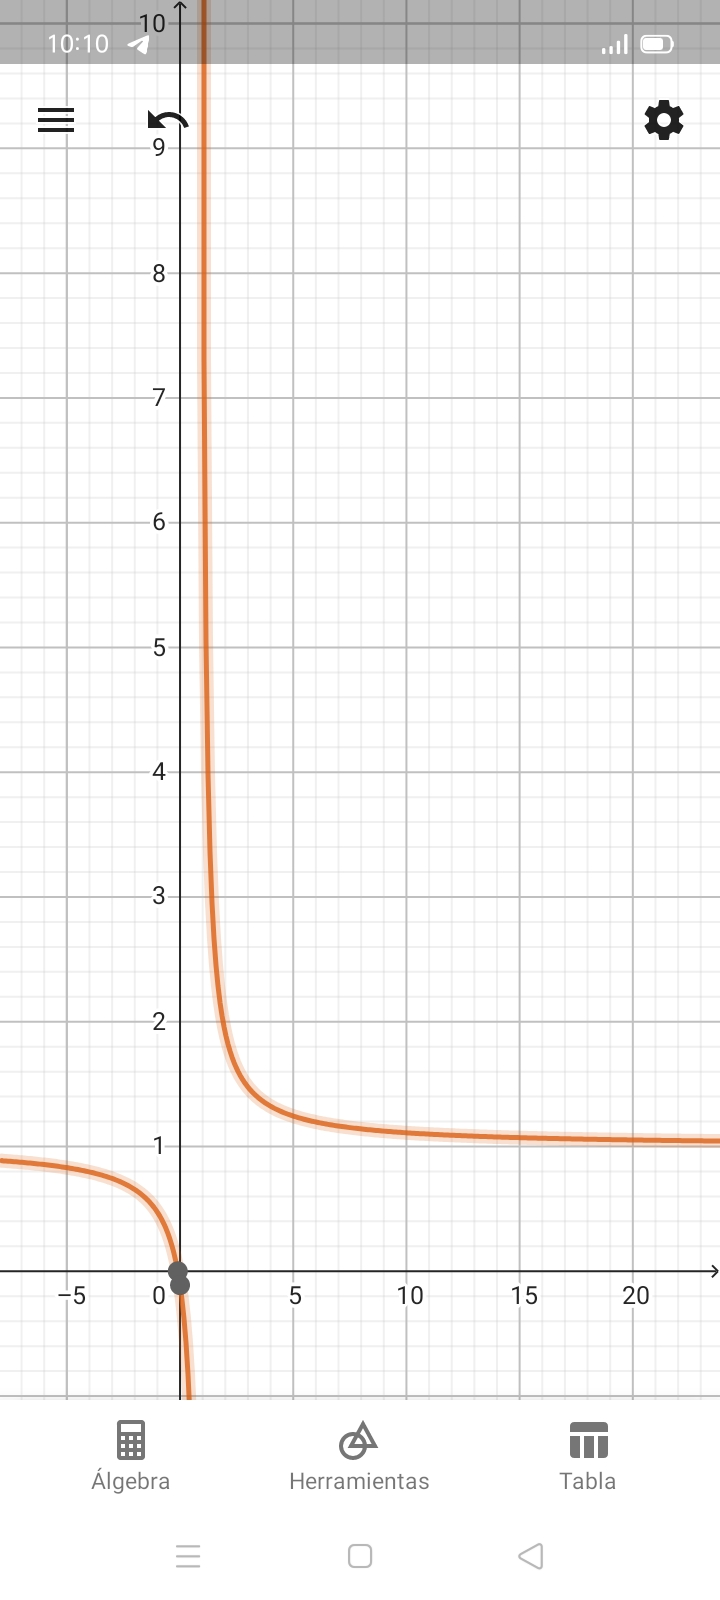
\includegraphics[scale=0.2]{Imagenes/b_1.jpg}\\
  B=75\\
  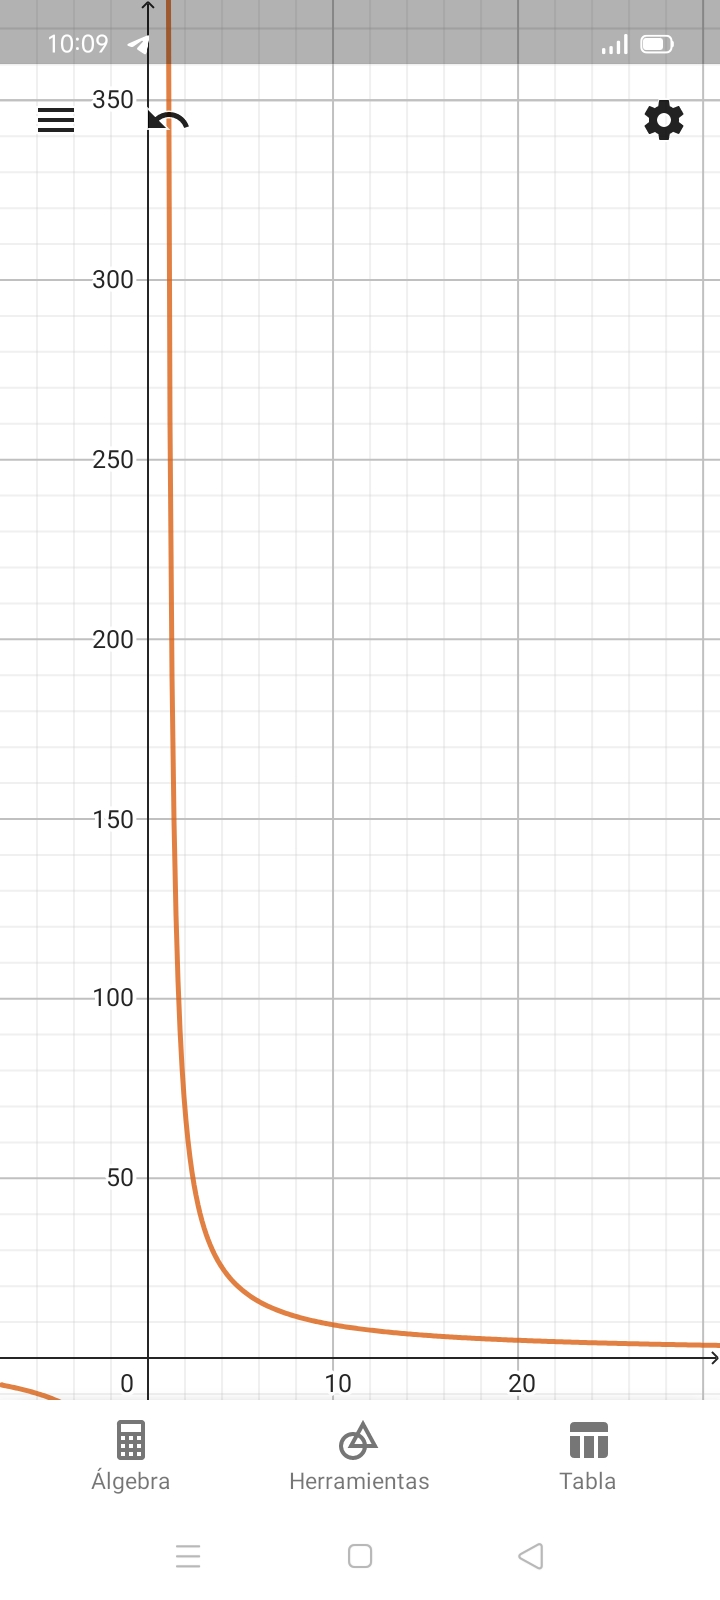
\includegraphics[scale=0.2]{Imagenes/b_75.jpg}\\
  B=500\\
  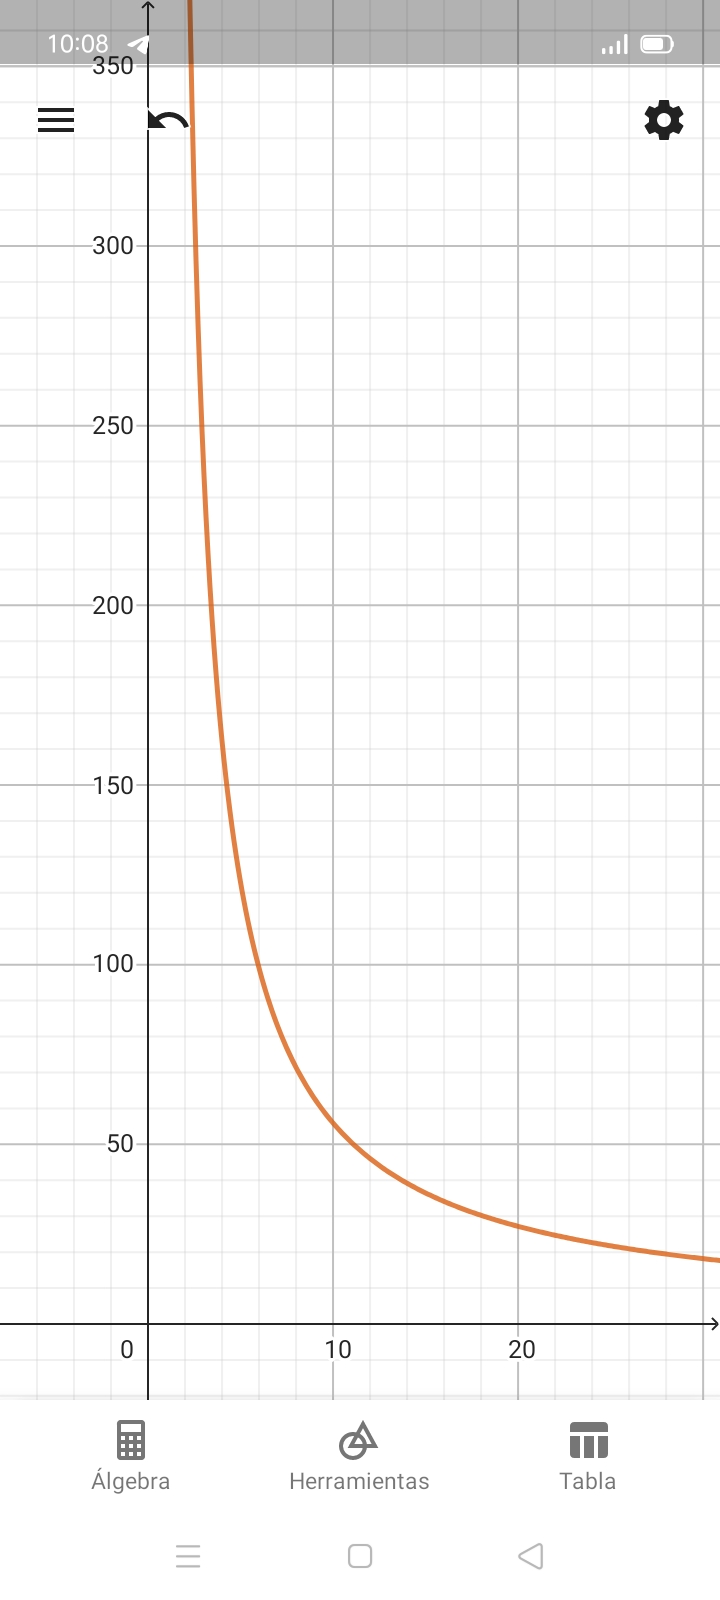
\includegraphics[scale=0.2]{Imagenes/b_500.jpg}\\
  B=1500\\
  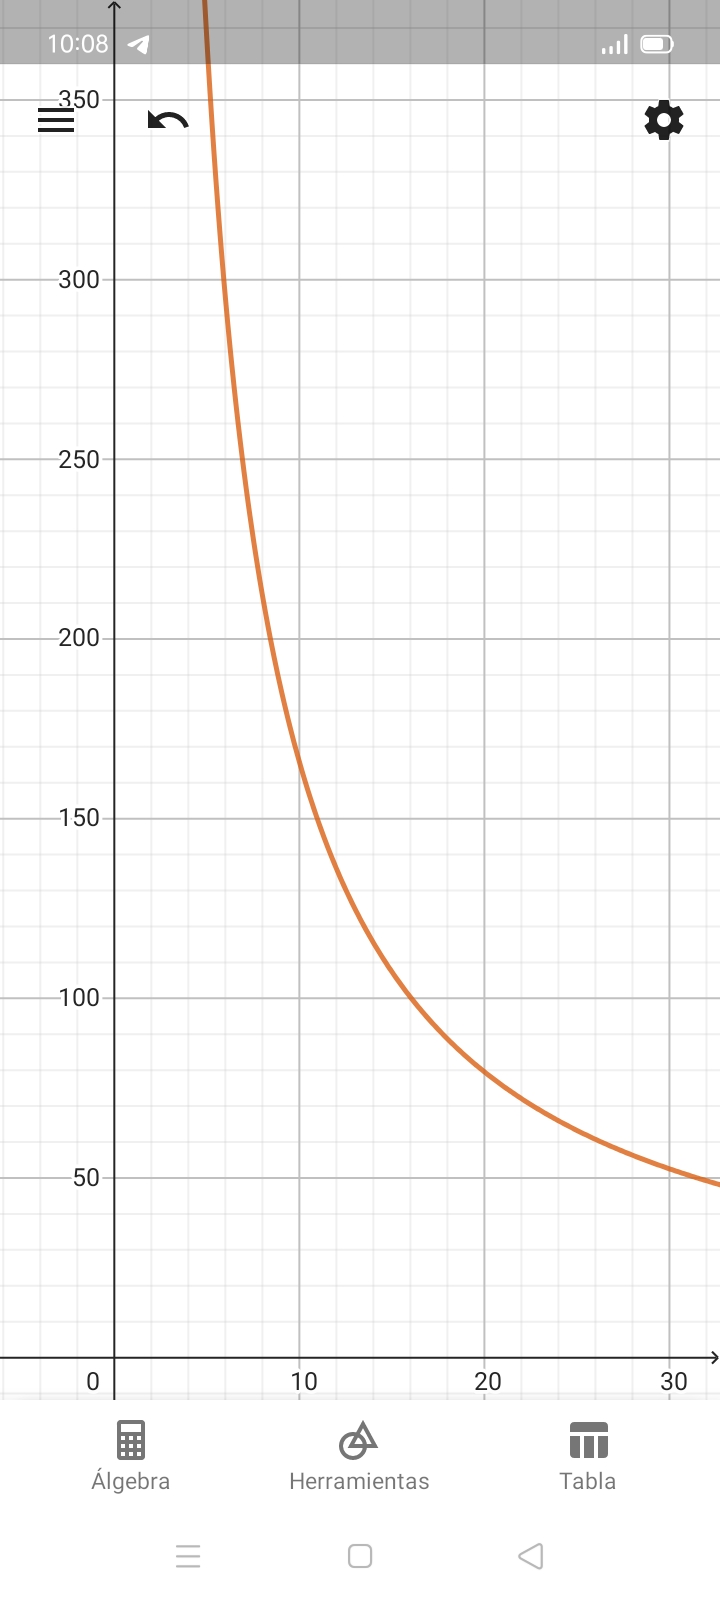
\includegraphics[scale=0.2]{Imagenes/b_1500.jpg}\\
\end{center}

\begin{table}[hb]
  \centering
  \caption{Tabla de valores aproximados para A = 0.9 y B variable:}
  \medskip
    \begin{tabular}{*{5}{p{3cm}}}
      Valor de B & Cercania = 1 & Cercania = 2 & Cercania = 5 & Cercania = 10 \\
      B = 1 & 11 & 1.90 & 1.24 & 1.11 \\
      B = 75 & 751 & 69 & 19 & 9 \\
      B = 500 & 5001 & 455 & 122 & 55 \\
      B = 1500 & 15001 & 1364 & 366 & 165 \\
    \end{tabular}
\end{table}

\subsubsection{De la clase SearchItem:}
Agregué un constructor copia. Crea un objeto a de esta clase a partir de copiar el contenido de otro objeto de esta misma clase.\\
Con motivo de poder intercambiar variables a la hora de ordenar en la clase Sorter.\\

\subsubsection{De la clase SearchResult:}
No realicé modificaciones sobre esta clase.\\

\subsubsection{De la clase Snippet:}
El miembro SnippetLength establece la longitud del snippet, es decir, la cantidad de términos que serán mostrados.\\
El método GetSnippet(string query,Documento doc,Regla regla) computa el snippet del documento dado en correspondencia con la query y los operadores establecidos en regla. Es conveniente recordar que para el cómputo del snippet solo se tienen en cuenta operadores * y \~{}.\\ 
El algoritmo para el cómputo del snippet tiene como idea central dividir el documento en subdocumentos con tantos términos como los definidos en SnippetLength. Como solo nos interesan los términos que aparecen en la query podemos desechar gran parte de los subdocumentos, y quedarnos con los que solo contienen algún término de query.  La forma en que hago esto es por cada término de la query que aparece en el documento, tomo cada una de las posiciones donde aparece y creo un subdocumento cuyo contenido son tantos términos como establece SnippetLength y distribuidos de tal forma que el término de la query quede como término central de ser posible. Como me interesa mostrar el contenido textual del documento como snippet y no solo los términos debo tener también en cuenta otra información como la posición en el texto que ocupan el primer y último término del subdocumento, ya que con estas posiciones puedo establecer los índices que delimitan en texto el contenido de mi snippet para calcularlo. De esta forma tengo una colección de subdocumentos y un listado de pares de posiciones. Debo decidir cual de los subdocumentos es el más relevante. Para ello utilizo el método Valorador.Valorar(queryDoc,subdocumentos,regla) que recibe como parámetros la query como un documento, la colección de subdocumentos y la regla, este método me devolverá un valor de relevancia para cada subdocumento. Luego basta con determinar el índice del subdocumento de mayor relevancia, y por cada elemento que esté entre las posiciones inicial y final agregarlo al snippet, que luego devuelvo.\\
Hay que notar que esta manera de computar el snippet es cómoda ya que se plantea el problema de una forma en la que es posible aprovechar el código escrito para el cálculo del score. \\

\subsubsection{De la clase Sorter:}
El método Sort(SearchItem[] items) ordena descendentemente por valor de score los resultados de la búsqueda. Utiliza el algoritmo insertion sort.\\
\begin{verbatim}
    Por cada prefijo del array(Los elementos desde el inicio (0) hasta una posición)
        Toma el ultimo elemento del prefijo.
        Mientras haya elementos antes que el y su score sea mayor (más importante) 
        que el elemento anterior intercámbialos.  
\end{verbatim}
Esto logra que en la iteración numero n por ejemplo tengamos los primeros n elementos del array ordenados descendentemente.\\

\subsubsection{De la clase Sugerencia:}
La clase Sugerencia mantiene dos miembros de datos que son modificados en otras partes del programa.\\
El miembro \_terminos que constituye los diferentes de la términos de la colección y que el método Coleccion.Inicializar() establece al ser llamado. De esta manera la asignación se realiza de forma única por ejecucion del programa. El método Inicializar(string[] terminos) es la vía por la cual Coleccion.Inicializar() hace la asignación.\\
El miembro \_token contiene los tokens de la consulta actual y es modificado en cada consulta del usuario ya que su contenido depende de la misma. El método Actualizar(string[] token) es la vía para modificar este miembro y es llamado desde el método Tokenizer.ProcesarQuery(string query).\\
De esta forma se consigue que la clase Sugerencia tenga toda la información necesaria para funcionar correctamente antes del llamado al método Sugerir().\\
El método Sugerir() devuelve una sugerencia para la consulta hecha por el usuario. Este método ignora todo token que no sea término. Luego por cada término en la consulta que no aparece en la colección de documentos elige entre todos los términos de la colección cual es el más similar y ese es el que sugiero. Para determinar la similaridad entre dos términos utilizo la EditDistance entre dos términos, conocida también como Distancia de Levenshtein.\\
El método EditDistance(string word1,string word2) computa la EditDistance entre estos dos string, que se define como el mínimo numero de operaciones de tipo :\\
\begin{enumerate}
  \item Insertar un caracter al final.
	\item Remover el caracter final.
	\item Igualar los caracteres finales.
\end{enumerate}
necesarias para hacer de los dos string iguales. Me decanto por una implementacion Bottom-Up del algoritmo.\\
Como curiosidad existe en LeetCode un problema llamado EditDistance que consiste en computar este valor entre dos palabras. Para probar mi algoritmo decidí enviarlo y resulto AC al primer \textcolor{blue}{\href{https://leetcode.com/submissions/detail/950932573/}{envío}}.\\

\subsubsection{De la clase Tokenizer:}
El método ProcesarTexto(string texto) normaliza el texto que recibe, más adelante se explicara en que consiste normalizar, y se auxilia del método Dividir(string texto) para extraer el listado de los términos y las posiciones donde aparece. Esta información es principalmente utilizada por el constructor de la clase Documento que recibe archivos.\\
El método Dividir(string texto) devuelve un listado de los términos que aparecen en el texto y las posiciones iniciales donde aparecen. Es un método de gran relevancia para la construcción de los documentos por la información que provee, note como dos miembros de la clase Documento son exactamente la salida de este método. Este método considera como término cualquier secuencia de caracteres entre dos espacios en blanco, notar como esto difiere de la definición de término dada más arriba. Es importante mencionar que la llamada a este método se realiza desde el método ProcesarTexto(string texto) y que el texto que se pasa a este método ya ha sido normalizado. El funcionamiento de este método es bastante intuitivo, primero se añade un espacio en blanco al final del texto para facilitar el procesamiento, luego cada caracter del texto o forma parte de un término, en cuyo caso se expande el actual, o es un espacio en blanco y constituye el final de un término. Como una nota si existen varios espacios en blanco consecutivos no se añaden términos vacíos al listado.\\
El método ProcesarQuery(string query) es de suma importancia para el programa. Él primeramente extrae los tokens de la consulta a través del método Tokenize(string texto), que devuelve solamente tokens validos (operadores o términos). Luego actualiza la clase Sugerencia a través del método Sugerencia.Actualizar(string[] token) con la información de la consulta actual, nótese que el contenido enviado a Sugerencia todavía contiene stop words como “la , los , de … ” y también contiene operadores, además de los términos. Luego se crea una nueva regla (objeto de la clase Regla) a partir de los tokens, que será utilizada posteriormente para el cálculo del score de documentos y el cómputo del snippet. Luego del listado se eliminan los términos que sean stop word, valiéndose del método Coleccion.EsStopWord(string termino), de esta forma no es necesario remover las stop word de la colección. Hay que notar que si las stop word se eliminan de la query en este paso, cuando se calcule posteriormente el score de los documentos estas no influirán en el mismo. \\
El método CrearTexto(string[] terminos) devuelve un texto que es la concatenación de los elementos de términos separados por espacios.\\
El método Tokenize(string texto) computa del texto dado un listado de tokens. Un token es :\\
\begin{enumerate}
  \item Uno de los símbolos ! \^{} \~{} *
	\item Una secuencia finita de letras y/o números.
\end{enumerate}
Los tokens se clasifican en dos categorías : Operadores (\~{} ! \^{} *) y Términos.\\
El proceso de computar los tokens es parecido al proceso por el cual Dividir(string texto) determina los diferentes términos. Cada caracter del texto o pertenece a un token o es el inicio de un nuevo token. Así se va creando un listado de tokens. Nótese que cada un de los símbolos ! \^{} * \~{} es un token de forma individual, el programa tiene en cuenta esto, de esta manera varios caracteres * consecutivos son tratados como tokens individuales , es el constructor de la clase regla quien se encarga luego de tratarlos como una unidad. Para llevar a cabo este algoritmo se cuenta con el método auxiliar AddToken(List<string> tokens, string token) que añade el token al listado solamente cuando es un token válido, se ofrecen métodos auxiliares también para determinar si un token es válido, si es operador, o si es término. Al finalizar el proceso de tokenizado se normaliza del listado de tokens aquellos que son términos para brindar así uniformidad a la consulta y consistencia con el estado de la colección.\\
El método EsTokenValido(string token) determina si un token es válido, es decir, si es operador o término.\\
El método EsTermino(string token) determina si un token es término a partir de la definición. Secuencia finita de letras y/o dígitos.\\
El método EsOperador(string token) determina si un token es operador a partir de la definición. Es uno de los símbolos \~{} ! \^{} *.\\
El método Normalizar(string texto, bool esTextoDeArchivo = false) es importante para el programa por proveer de uniformidad al contenido sobre el que se trabaja. Este método es simple, itera caracter a caracter aplicando las siguientes transformaciones:\\
\begin{enumerate}
  \item Convierta mayúsculas a minúsculas.
	\item Si la letra tiene tilde se convierte en su variante sin tilde.
	\item Si es texto de un archivo convierte todo caracter que no sea letra o dígito en espacios en 	blanco.
\end{enumerate}
La transformación 1 y 2 proporcionan uniformidad. La transformación 3 se ejecuta solo en archivos, pues de ejecutarse en consultas eliminaría los operadores, así se mantiene solo el contenido fundamental del archivo, aquel expresado por palabras y números.\\

\subsubsection{De la clase Valorador:}
El método Valorar(Documento query, Documento[] documentos,Regla regla) computa el score para cada documento dado con respecto a la query teniendo en cuenta además los operadores definidos por el usuario. Primero crea un vector a partir de la consulta y luego crea un vector a partir de cada documento. Luego aplica el operador * a la consulta. Por cada documento que cumpla con los requisitos de los operadores ! \^{}, aplicar el operador \~{} y calcular la similitud del vector de dicho documento con el vector de la consulta, esta similaridad es el score de dicho documento. Devolver los scores.\\
Anotaciones de este método:
\begin{itemize}
  \item Aplicar el operador * consiste en que a las componentes del vector de la consulta que corresponden con algún termino precedido por * multiplicarlas por un valor en función de la cantidad de *. La clase Regla proporciona una implementacion de esta función. Regla.CalcularShould(int cantidadDeAsteriscos). Notemos que al aplicar el operador * a la consulta   las componentes de dichos términos adquieren un valor mayor y por tanto se vuelven más relevantes.
  \item Aplicar el operador ! consiste en ignorar a los documentos que contengan alguno de los términos precedidos por este operador en la consulta, pues no deben contener ninguno.
  \item Aplicar el operador \^{} consiste en ignorar a los documentos que no contengan alguno de los términos precedidos por este operador en la consulta, pues deben aparecer todos.
  \item Aplicar el operador \~{} consiste en por cada pareja de términos relacionados por este operador multiplicar sus componentes en el vector del documento por un valor en función de la cercanía de dichos términos en el documento. De estar muy cercanos adquieren mayor relevancia en comparación con otros términos de la consulta, además aumentan el score general del documento. La clase Regla.CalcularClose(int cercania) calcula el valor en fución de la cercanía. La cercania es calculada a partir del método auxiliar Documento.Cercania(string terminoA,string terminoB). Por esta razón es conveniente que este método reciba los documentos y no los vectores de los mismos. Es la clase Documento quien se encarga de computar la cercanía porque las funcionalidades y la información necesaria para esta tarea están contenidas dentro de dicha clase. No tiene sentido aplicar el operador de cercanía en el vector de la query, necesariamente los términos son cercanos.
\end{itemize}
El método Similaridad(Vector u,Vector v) encapsula la función para el calculo de la similitud entre dos vectores. En este caso hace una llamada al método SimilaridadCoseno(Vector u,Vector v).\\
El método SimilaridadCoseno(Vector u,Vector v) calcula la similaridad entre dos vectores a partir de la fórmula establecida en la figura 3 del documento \textcolor{blue}{\url{http://ccdoc-tecnicasrecuperacioninformacion.blogspot.com/2012/12/modelo-vectorial.html}}\\
\begin{equation}
  SimCos(d_{(d)},q) = \frac {\sum_{n=1} (P_{(n,d)} \times P_{(n,q)})}  {\sqrt{\sum_{n=1} (P_{(n,d)})^2 \times \sum_{n=1} (P_{(n,q)})^2}}
\end{equation}
El numerador de esta fórmula representa el producto vectorial del vector documento y el vector consulta, el denominador representa la raíz cuadrada aritmética del producto de la norma del vector documento por la norma del vector consulta. La norma de un vector calculada como el producto vectorial de un vector por si mismo.\\
La decisión de establecer esta fórmula para el cálculo de la similaridad como valor de score proviene de haber probado distintos enfoques y comparar sus resultados ante diferentes consultas. Este fue el más sobresaliente. Otros enfoques que probé fueron calcular el score de un documento como la suma de los score individuales de cada término de la consulta respecto al documento; también utilizando una formula similar a la de arriba pero sin raíz cuadrada en el denominador y sumando en vez de multiplicar.\\
El método Pesar(string termino,Documento documento) es utilizado a la hora de crear los vectores para los documentos y la consulta y establece el valor de la componente asociada al término como el valor tf-idf de ese término en el documento.\\
El método Idf(string termino) devuelve el valor idf del término con respecto a la colección, que es una medida de cuan común es este termino en la colección. La fórmula para calcularlo se basa en la entrada de Wikipedia de \textcolor{blue}{\href{https://es.wikipedia.org/wiki/Tf-idf}{Tf-Idf}}.\\
\begin{equation}
  idf(t,D) = \log{\frac{|D|}{\{d \in D : t \in d\}}}
\end{equation}
El método Tf(string termino,Documento documento) devuelve el valor de tf del término en el documento que es una medida de cuan frequente es el término en el documento. Para esto calcula su frecuencia normalizada.\\
Los métodos FrecuenciaNormalizada(string termino,Documento documento) y FrecuenciaBruta(string termino,Documento documento) proveen la forma de calcular la frecuencia normalizada de un término en el documento a través de la fórmula :\\
\begin{equation}
  tf(t,d)=\frac {f(t,d)} {max\{f(t,d):t \in d\}}
\end{equation}
La frecuencia normalizada evita una predisposición hacia documentos largos.\\
Hay que notar que en el cálculo de la frecuencia normalizada el denominador en el caso de mi programa es la frecuencia del término del documento de mayor frecuencia y que no es stop word. De esto se encarga la propiedad Documento.MostFrequentCount.\\

\subsubsection{De la clase Vector:}
El miembro \_vector representa el contenido del vector como un diccionario donde las llaves son los términos y los valores son el valor tf-idf del termino. Puede decirse que cada par <llave,valor> es una componente del vector, y que si para término dado, el no aparece en el vector es porque el valor de su componente es cero, esta es una definición a conveniencia para hacer más eficaz la implementación.\\
El constructor r.Vector(Documento documento) crea un vector a partir de un documento asociando a cada término único del documento con su valor tf-idf en el documento, para esto se auxilia del método Valorador.Pesar(string termino,Documento documento)\\
Los constructores Vector(Vector other) y Vector(Dictionary<string,double> otherVectorContent)  crean un vector a partir de otro vector.\\
El indizador de la clase Vector recibe como parámetro un término y devuelve el valor de tf-idf asociado a ese término, devuelve 0 si el término no aparece, de esta manera se hacen cómodas las operaciones de multiplicar vectores como veremos adelante.\\
La propiedad Dimension devuelve la cantidad de términos diferentes que componen el vector. Aunque realmente la dimensión del vector es la cantidad de términos diferentes que componen la colección.\\
La propiedad Terminos devuelve una copia de los términos que forman el vector.\\
La propiedad Contenido devuelve una copia del miembro \_vector.\\
El operador sobrecargado *(Vector u,Vector v) implementa el producto punto entre dos vectores. Este producto es un escalar y se calcula como la suma de los productos de las componentes de los vectores. Hay que notar que para efectuar este producto se recorren los distintos términos que componen alguno de los vectores, el de menor cantidad para mayor eficacia, y se suma el producto de los valores de ambos vectores asociados a este termino. Si un termino aparece en un vector y en el otro no entonces en el que no aparece toma valor 0 por lo que al multiplicar no aporta nada a la suma, que es lo deseado.\\
El operador sobrecargado +(Vector u,Vector v) implementa la suma de vectores, que es la suma componente a componente.\\
El método AplicarOperador(string index,double value) es un método auxiliar que permite modificar el valor de una componente del vector, la asociada al termino index. A este valor se le multiplica por value. De esta forma se consigue aplicar los operadores * \~{} a términos específicos.\\
El método ToString() se sobrescribe para fines de depuración.\\

\end{document}
